






%\chapter*{Part I Conclusion}{Introduction de la Partie I}
\chapter*{\bpar{Conclusion of Part I: a definition of co-evolution}{Conclusion de la Partie I : une définition de la co-évolution}}


% to have header for non-numbered introduction
% \markboth{Conclusion of Part I}{Conclusion of Part I}
\markboth{Conclusion de la Partie I}{Conclusion de la Partie I}


%\headercit{}{}{}


%La première conclusion marquante de cette première partie se résume parfaitement dans le meme suivant :


%{\centering
%\medskip
%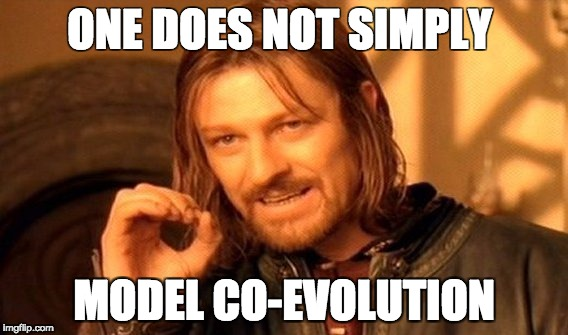
\includegraphics[width=\textwidth]{Figures/Art/onedoesnotsimply.jpg}
%\medskip
%}


\bpar{
This first part allows us to formulate much more precisely our research question. Indeed, the first chapter allowed us to draw a sketch of the diversity of processes involved and of the temporal and spatial scales concerned. The second chapter gave us a very general view of existing modeling approaches and of their precise scientific context. Finally, the third chapter positions the question in an epistemological way, shed some light on co-evolution through a multi-disciplinary perspective, and clarifies the complexity with which we are dealing. It allows us to open on the directions to take in order to lead successfully the project of modeling the co-evolution.
}{
Cette première partie nous permet de cerner bien plus précisément notre question de recherche. En effet, le premier chapitre nous a permis de dresser un portrait de la diversité des processus impliqués et des échelles temporelles et spatiales concernées. Le deuxième chapitre nous a donné une vue très générale des modélisations existantes et de leur contexte scientifique précis. Enfin, le troisième chapitre positionne la question de manière épistémologique, apporte un éclairage multi-disciplinaire sur la co-évolution, et clarifie la complexité dans laquelle nous nous situons. Cela nous permet d'ouvrir sur les directions à prendre par la suite pour mener à bien l'entreprise de modélisation de la co-évolution.
}


\subsection*{Defining co-evolution}{Définir la co-évolution}


\bpar{
After the literature review given in~\ref{sec:modelingsa}, that includes different degrees of coupling between components of networks and territories, we are first able to precise what will be meant by \emph{modeling co-evolution}, by giving a definition of co-evolution in view of the multidisciplinary overview given in~\ref{sec:epistemology}.
}{
Après l'aperçu de la littérature donné en~\ref{sec:modelingsa}, incluant différents degrés de couplage entre les composantes des réseaux et territoires, nous sommes tout d'abord en mesure de préciser ce que nous entendrons par \emph{modéliser la co-évolution}, en fixant une définition de la co-évolution au regard de l'aperçu multidisciplinaire mené en~\ref{sec:epistemology}.
}


\bpar{
We propose the following entry for the specific case of transportation networks and territories, which echoes to the three main points (existence of evolutive processes, definition of entities or populations, isolation of subsystems in space and time) that we gave in~\ref{sec:epistemology}. It verifies the three following specifications.
}{
Nous proposons l'entrée suivante pour le cas spécifique des réseaux de transport et des territoires, qui fait écho au trois points essentiels (existence de processus évolutifs, définition des entités ou des populations, isolation de sous-systèmes dans le temps et l'espace) que nous avons dégagé en~\ref{sec:epistemology}. Celle-ci vérifie les trois spécifications suivantes.
}


\bpar{
First of all, evolutive processes correspond to transformations of components of the territorial system at the different scales: transformation of cities on the long time, of their networks, transmission between cities of socio-economic characteristics carries by microscopic agents but also cultural transmission, reproduction and transformation of agents themselves (firms, households, operators)\footnote{This list is based on assumptions of the evolutive urban theory that we already briefly introduced and that we will develop in itself in Chapter~\ref{ch:evolutiveurban}. It can not be exhaustive, since what would be the ``ADN of a city'' remains an open question as recalls \noun{Denise Pumain} in a dedicated interview~\ref{app:sec:interviews}.}.
}{
Dans un premier temps, les processus évolutifs correspondent aux transformations des composantes du système territorial aux différentes échelles : transformation sur le temps long des villes, de leurs réseaux, transmission entre villes des caractéristiques socio-économiques portées par les agents microscopiques mais aussi transmission culturelle, reproduction et transformation des agents eux-mêmes (firmes, ménages, opérateurs)\footnote{Cette liste s'appuie sur les hypothèses de la théorie évolutive des villes que nous avons déjà introduite brièvement et que nous développerons à part entière en Chapitre~\ref{ch:evolutiveurban}. Elle ne peut être exhaustive, puisque ce qui ferait ``l'ADN d'une ville'' reste une question ouverte comme nous le rappelle \noun{Denise Pumain} dans un entretien dédié~\ref{app:sec:interviews}.}.
}



\bpar{
These evolutive processes may imply a co-evolution. Within a territorial system, can simultaneously co-evolve: (i) given entities (a given infrastructure and given characteristics of a given territory for example, i.e. individuals), when their mutual influence will be circularly causal (at the corresponding scale); (ii) populations of entities, what will be translated for example as such type of infrastructure and given territorial components co-evolve at a statistical level in a given geographical region; (iii) all the components of a system at a small geographical scale when there exists strong global interdependencies. Our approach is thus fundamentally \emph{multi-scale} and articulates different significations at different scales.
}{
Ces processus évolutifs peuvent impliquer une co-évolution. Au sein d'un système territorial, pourront être en co-évolution à la fois : (i) des entités données (telle infrastructure et telles caractéristiques de tel territoire par exemple, c'est-à-dire des individus), lorsque leur influence mutuelle sera circulairement causale (à l'échelle leur correspondant) ; (ii) des populations d'entités, ce qui se traduira par exemple par tel type d'infrastructure et telle composante territoriale co-évoluent au niveau statistique dans une région géographique donnée ; (iii) l'ensemble des composantes d'un système à petite échelle géographique lorsqu'il existe de fortes interdépendances globales. Notre vision est donc fondamentalement \emph{multi-échelles} et articule différentes significations à différentes échelles.
}


\bpar{
Finally, the constraint of an isolation implies, in relation with the previous point, that co-evolution and the articulation of significations will have a meaning if there exists spatio-temporal isolations of subsystems in which differente co-evolutions operate, what is directly in accordance with a vision in \emph{Multi-scalar systems of systems}.
}{
Enfin, la contrainte d'une isolation implique, en lien avec le point précédent, que la co-évolution et l'articulation des significations auront un sens s'il existe des isolations spatio-temporelles de sous-systèmes où s'effectuent les différentes co-évolutions, ce qui est en accord direct avec un vision en \emph{Systèmes de systèmes multi-échelles}.
}


% dernier point : lien avec la notion de morphogenese : a appuyer dans intro de II

\bpar{
This extended definition will constitute our reference in the following when we will evoke the co-evolution of transportation networks and territories.
}{
Cette définition élargie constituera notre référence par la suite lorsqu'on parlera de co-évolution des réseaux de transport et des territoires.
}

%L'une de nos contributions en synthèse faite en~\ref{sec:theory} sera de formaliser cette définition au regard des résultats que nous aurons obtenus. Elle constituera jusque là notre base d'investigation.


\bpar{
We can then synthesize the fundamental results of this first part in the two following significant facts:
\begin{enumerate}
	\item The hypothesis of co-evolution of transportation networks and territories is supported from a theoretical and thematic point of view, et we construct a precise definition for it.
	\item Co-evolution remains relatively poorly explored in the literature of urban modeling, the characteristic of concerned disciplines and their interactions being a potential cause for it.
\end{enumerate}
}{
Nous pouvons alors synthétiser les résultats fondamentaux de cette première partie dans les deux faits marquants suivants :
\begin{enumerate}
	\item L'hypothèse de la co-évolution des réseaux de transport et des territoires est supportée d'un point de vue théorique et thématique, et nous en construisons une définition précise.
	\item La co-évolution reste très peu explorée dans la littérature de modélisation urbaine, les caractéristiques des disciplines concernées et leurs interactions pouvant en être une cause.
\end{enumerate}
}


\bpar{
We develop now the perspective that open at this stage.
}{
Développons à présent les perspectives qui s'ouvrent à ce stade.
}

\subsection*{On the need of an empirical characterization}{Du besoin d'une caractérisation empirique}


\bpar{
The broadest signification, i.e. generalized interdependency, is rapidly limited if its patterns are not finely characterized. It allows as an epistemological premise to consider certain ontologies and certain modeling approaches, but allows difficultly to finely understand the structure and processes of a system. The object will be then to decrease in generality and consider subsystems, in which we can consider the co-evolution of entities and of population. An understanding at this level necessitates a fine empirical characterization, without which our distinction would have no sense. A question that opens, and that we will tackle in the following, is then which are the possible empirical methods to characterize a co-evolution between entities or populations of entities.
}{
La signification la plus large, c'est-à-dire l'interdépendance généralisée, trouve vite ses limites si les motifs ne sont pas finement caractérisés. Elle permet comme prémisse épistémologique de considérer certaines ontologies et certaines démarches de modélisation, mais permet difficilement de comprendre finement la structure et les processus d'un système. Il s'agira alors de descendre en généralité et de considérer des sous-systèmes, au sein desquels on peut s'intéresser à la co-évolution d'entités et de population. Une compréhension à ce niveau nécessite une caractérisation empirique fine, sans quoi notre distinction n'aurait pas de sens. Une question qui s'ouvre, et que nous devrons traiter par la suite, est alors quelles sont les méthodes empiriques possibles pour caractériser une co-évolution entre entités ou populations d'entités.
}



\subsection*{Two complementary tracks}{Deux pistes complémentaires}


% combiner : empirique (carac empirique) et modeling / deux echelles (plusieurs, mais au min deux) / deux stream d'inclusion dans les modeles : idem ? / coevol amene deja l'idee d'isolation et de sous systeme indep : morphogenesis
%  -> unexplored streams from the literature - details why particularly suited in intro Part II . objectif de l'inclusion dans les modèles


\bpar{
The state of the art done in~\ref{sec:modelingsa} above witnesses a weakness in the literature in the domain of strong coupling between the evolution of territories and network growth, given the restricted range and the disparity of reviewed works. The gap to fill on this point would thus be linked to the introduction of models strongly coupled in time more or less multi-processes and multi-scale, for which a part of the models described in~\ref{sec:modelingsa} then in~\ref{sec:modelography} are precursors.
}{
L'état de l'art fait en~\ref{sec:modelingsa} ci-dessus témoigne d'une faiblesse de la littérature dans le domaine du couplage fort entre évolution des territoires et croissance des réseaux, vu la portée restreinte et la disparité des travaux revus. Les lacunes à combler sur ce point seraient donc liées à l'introduction de modèles fortement couplés dans le temps plus ou moins multi-processus et multi-échelles, pour lesquels une partie des modèles décrits en~\ref{sec:modelingsa} puis en~\ref{sec:modelography} sont précurseurs.
}



\bpar{
The first exploratory research we will lead will have to answer to different conceptual tensions that result from the conclusions we just obtained:
\begin{itemize}
	\item allowing both an empirical approach, and more particularly a characterization method, and a modeling approach;
	\item allowing to take into account different scales;
	\item allowing the inclusion of ontologies for territories and for networks that are not always directly compatible.
\end{itemize}
}{
Les premières recherches exploratoires que nous allons mener doivent répondre à différentes tensions conceptuelles qui découlent des conclusions que nous venons de tirer :
\begin{itemize}
	\item permettre à la fois une approche empirique, et en particulier un méthode de caractérisation, ainsi qu'une approche de modélisation ;
	\item permettre la prise en compte de différentes échelles ;
	\item permettre l'inclusion d'ontologies pour les territoires et pour les réseaux qui ne sont pas toujours directement compatibles.
\end{itemize}
}


\bpar{
The scales will especially be a mesoscopic and a macroscopic scale since as we suggested in~\ref{sec:reproducibility} with the study of traffic flows, and as shows \cite{yasmin2017macro} for the validation of an activity model, the microscopic scale witnesses complex trajectories that are difficult to reproduce.
}{
Les échelles seront notamment une échelle mesoscopique et une échelle macroscopique puisque comme nous l'avons suggéré en~\ref{sec:reproducibility} avec l'étude des flux de trafic, et comme le montre \cite{yasmin2017macro} pour la validation d'un modèle d'activités, l'échelle microscopique présente des trajectoires complexes difficiles à reproduire.
}


\bpar{
We will choose to answer simultaneously to these different problematics with an original strategy of a double thematic entry.
}{
Nous choisirons pour répondre simultanément à ces différentes problématiques une stratégie originale de double entrée thématique.
}


% why does not study mobility et suggestion preliminaire de meso-macro scales only. -> conclusion Partie I
%\bpar{}
%{
%Il faut aussi garder à l'esprit que le transport en lui-même est différent des réseaux de transport\comment[FL]{en quoi estce un argument ?}, puisqu'il correspond à l'utilisation de ceux-ci par les agents territoriaux. Dans une grande partie des approches que nous décrirons par la suite, et typiquement les approches appliquée en planification urbaine, la modélisation du transport s'axe sur des question de demande, d'offre, de congestion, c'est-à-dire à des échelles relatives à la mobilité, et est liée au réseau mais ne se concentre pas directement sur celui-ci\comment[FL]{ce n'est pas clair $\rightarrow$ la croissane du reseau ?, l'usage du reseau ? la croissance de l'usage du reseau ?} comme notre positionnement propose\comment[AB]{$\simeq$}.
%}


